
% V_Results_and_Discussion/V_E_Force_Performance.tex
% English AIAA manuscript subsection
% Included by main.tex using:
% 
% V_Results_and_Discussion/V_E_Force_Performance.tex
% English AIAA manuscript subsection
% Included by main.tex using:
% 
% V_Results_and_Discussion/V_E_Force_Performance.tex
% English AIAA manuscript subsection
% Included by main.tex using:
% 
% V_Results_and_Discussion/V_E_Force_Performance.tex
% English AIAA manuscript subsection
% Included by main.tex using:
% \input{V_Results_and_Discussion/V_E_Force_Performance}

\subsection{Aerodynamic Coefficient Prediction Performance}
\label{subsec:aerodynamic-coefficient-prediction}

Accurate reconstruction of the surface pressure field does not, by itself, guarantee accurate prediction of integrated aerodynamic coefficients. The latter requires a downstream model to extract the load-relevant information from a high-dimensional pressure representation. The force-label efficiency of this representation is examined using three coefficient-regression strategies: direct regression from geometry and flow conditions (D0), regression conditioned on the pressure field predicted by the fixed M2 model (D1), and regression conditioned on CFD-reference pressure (D2). Separate regressors are trained for the lift coefficient $C_L$, drag coefficient $C_D$, and pitching-moment coefficient $C_{M_z}$. Seven force-label budgets, $N=10$, 20, 30, 40, 50, 80, and 100 wings, are considered, with three independently sampled training subsets at each budget. All reported errors are evaluated on the same 88 test wings. Here $N$ denotes the number of wings used to train the downstream coefficient regressors; the pressure supervision previously used to establish the fixed M2 model is not included in this budget. Figure~\ref{fig:ve-force-mae} shows the mean absolute error (MAE) across the seven budgets, and Table~\ref{tab:ve-force-mae} provides the corresponding numerical comparisons.

\begin{figure*}[!t]
    \centering
    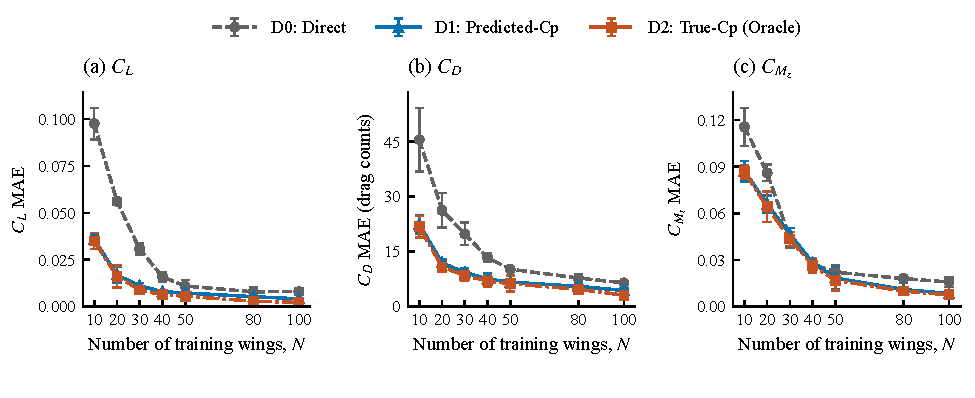
\includegraphics[width=0.96\textwidth]{V_Results_and_Discussion/figures/V_E_Fig25/V_E_Fig25_ve_force_mae.pdf}
    \caption{Force-coefficient MAE versus training size: (a) $C_L$, (b) $C_D$, and (c) $C_{M_z}$. D0, D1, and D2 use geometry/flow, M2-predicted pressure, and CFD pressure, respectively .}
    \label{fig:ve-force-mae}
\end{figure*}

The pressure-conditioned model provides its largest practical benefit at low force-label budgets. At $N=20$, the MAEs of D0 for $C_L$, $C_D$, and $C_{M_z}$ are 0.05610, 26.27 drag counts, and 0.08609, respectively. With M2-predicted pressure as additional input, D1 reduces these values to 0.01680, 11.88 drag counts, and 0.06592, corresponding to reductions of 70.1\%, 54.8\%, and 23.4\%. The improvement is strongest for lift, whose integrated response is directly related to the surface pressure loading. The reduction in drag-coefficient error is also substantial. By comparison, the smaller gain in pitching moment suggests a less favorable mapping from the available pressure representation to that particular integrated response; the present experiments do not isolate the physical origin of this difference.

Across the investigated budgets, the MAE generally decreases as more force-labeled wings become available, while the benefit of pressure conditioning remains coefficient-dependent. D1 outperforms D0 in mean MAE at all seven budgets for $C_L$ and $C_D$. For $C_{M_z}$, however, D1 is slightly less accurate at $N=30$ and 40: its MAEs are 0.04664 and 0.02833, compared with 0.04419 and 0.02746 for D0. At $N=100$, D1 reaches MAEs of 0.00414 for $C_L$, 4.39 drag counts for $C_D$, and 0.00838 for $C_{M_z}$. These results demonstrate that the contribution of the intermediate pressure field is not uniform across the three coefficients or training budgets.

The D2 results help distinguish the information supplied by pressure from the ability of the downstream regressor to use it. At $N=20$, replacing predicted pressure with CFD-reference pressure yields only modest additional reductions, to MAEs of 0.01611, 10.83 drag counts, and 0.06422 for $C_L$, $C_D$, and $C_{M_z}$, respectively. The separation becomes more apparent at $N=100$, where D2 achieves 0.00220, 3.12 drag counts, and 0.00755, compared with 0.00414, 4.39 drag counts, and 0.00838 for D1. Thus, additional pressure fidelity is more effectively reflected in the coefficient estimates when more force-labeled examples are available. This observation is consistent with a limitation imposed by downstream regression under very small training budgets, although the present comparison does not establish that explanation uniquely. Furthermore, D1 and D2 are fitted separately, so their difference cannot be attributed solely to M2 pressure error. Because D2 requires CFD-reference pressure as an input, it is a diagnostic reference rather than a deployable geometry-to-force surrogate.

The MAE over all 88 wings is complemented in Table~\ref{tab:ve-force-mae} by Best90 and Best80 MAE, which average the 80 and 71 lowest absolute errors, respectively, within each evaluated model. At $N=20$, D1 gives a drag MAE of 11.88 counts over all test wings, compared with Best90 and Best80 values of 8.98 and 7.30 counts. The corresponding D0 values are 26.27, 20.74, and 17.26 counts. Hence, the improvement from pressure conditioning is also evident over the lower-error majority of the test wings, rather than being restricted to changes in a few high-error cases. The gap between the full and trimmed means nevertheless indicates an uneven distribution of errors across wing configurations. Since the wings retained by the Best90 and Best80 definitions can differ between models, these statistics characterize error concentration and do not replace the full-set MAE.

\begin{table*}[!t]
    \centering
    \caption{Force-coefficient MAEs on 88 test wings, averaged over three training subsets.}
    \label{tab:ve-force-mae}
    \begingroup
    \fontsize{8.2}{9.8}\selectfont
    \setlength{\tabcolsep}{3.0pt}
    \renewcommand{\arraystretch}{1.06}

    \begin{tabular}{@{}r*{9}{c}@{}}
    \hline
    & \multicolumn{3}{c}{MAE}
    & \multicolumn{3}{c}{Best90 MAE}
    & \multicolumn{3}{c}{Best80 MAE} \\
    $N$ & D0 & D1 & D2
        & D0 & D1 & D2
        & D0 & D1 & D2 \\
    \hline

    \multicolumn{10}{@{}l}{\textit{$C_L$ (dimensionless)}} \\
    10  & 0.09764 & 0.03584 & 0.03501 & 0.08258 & 0.02785 & 0.02726 & 0.07027 & 0.02315 & 0.02260 \\
    20  & 0.05610 & 0.01680 & 0.01611 & 0.04473 & 0.01295 & 0.01211 & 0.03673 & 0.01055 & 0.00978 \\
    30  & 0.03067 & 0.01113 & 0.00889 & 0.02520 & 0.00903 & 0.00708 & 0.02082 & 0.00729 & 0.00568 \\
    40  & 0.01592 & 0.00791 & 0.00626 & 0.01263 & 0.00620 & 0.00484 & 0.01015 & 0.00511 & 0.00398 \\
    50  & 0.01095 & 0.00729 & 0.00557 & 0.00793 & 0.00563 & 0.00429 & 0.00647 & 0.00455 & 0.00346 \\
    80  & 0.00787 & 0.00529 & 0.00287 & 0.00558 & 0.00411 & 0.00218 & 0.00444 & 0.00347 & 0.00182 \\
    100 & 0.00800 & 0.00414 & 0.00220 & 0.00580 & 0.00335 & 0.00174 & 0.00478 & 0.00274 & 0.00145 \\

    \hline
    \multicolumn{10}{@{}l}{\textit{$C_D$ (drag counts)}} \\
    10  & 45.56 & 22.44 & 21.82 & 38.36 & 17.33 & 16.83 & 32.99 & 14.55 & 14.20 \\
    20  & 26.27 & 11.88 & 10.83 & 20.74 & 8.98 & 8.17 & 17.26 & 7.30 & 6.76 \\
    30  & 19.83 & 9.33 & 8.47 & 15.21 & 6.21 & 5.56 & 12.41 & 4.65 & 4.37 \\
    40  & 13.34 & 7.54 & 7.00 & 9.95 & 4.70 & 4.40 & 8.01 & 3.51 & 3.42 \\
    50  & 10.20 & 6.67 & 6.26 & 7.15 & 3.81 & 3.47 & 5.62 & 2.76 & 2.62 \\
    80  & 7.79 & 5.51 & 4.69 & 4.96 & 3.29 & 2.61 & 3.87 & 2.38 & 1.97 \\
    100 & 6.47 & 4.39 & 3.12 & 4.73 & 2.93 & 2.18 & 3.79 & 2.21 & 1.70 \\

    \hline
    \multicolumn{10}{@{}l}{\textit{$C_{M_z}$ (dimensionless)}} \\
    10  & 0.11566 & 0.08714 & 0.08674 & 0.09678 & 0.07124 & 0.07112 & 0.08294 & 0.05965 & 0.05956 \\
    20  & 0.08609 & 0.06592 & 0.06422 & 0.07016 & 0.05444 & 0.05251 & 0.06067 & 0.04643 & 0.04434 \\
    30  & 0.04419 & 0.04664 & 0.04351 & 0.03604 & 0.03874 & 0.03608 & 0.02976 & 0.03283 & 0.03051 \\
    40  & 0.02746 & 0.02833 & 0.02650 & 0.02139 & 0.02264 & 0.02140 & 0.01756 & 0.01881 & 0.01796 \\
    50  & 0.02210 & 0.01837 & 0.01695 & 0.01680 & 0.01481 & 0.01363 & 0.01394 & 0.01202 & 0.01136 \\
    80  & 0.01800 & 0.01098 & 0.00997 & 0.01326 & 0.00874 & 0.00826 & 0.01109 & 0.00735 & 0.00701 \\
    100 & 0.01574 & 0.00838 & 0.00755 & 0.01146 & 0.00681 & 0.00632 & 0.00984 & 0.00576 & 0.00537 \\

    \hline
    \end{tabular}
    \endgroup
\end{table*}

The representative small-sample case in Fig.~\ref{fig:ve-force-parity} provides a complementary view of the error distribution. At $N=20$, D1 predictions for lift and drag lie appreciably closer to the ideal agreement line than those of D0; the pitching-moment predictions remain more dispersed, consistent with their smaller relative MAE reduction. To prevent repeated evaluations of the same wing from appearing as independent observations, each plotted prediction is the arithmetic mean of the outputs from the three training-subset models for that wing. This averaging is used only for visualization: the metrics in Fig.~\ref{fig:ve-force-mae} and Table~\ref{tab:ve-force-mae} are calculated separately for each training subset before aggregation. Taken together, the results indicate that the fixed hierarchical pressure representation improves coefficient estimation when force labels are scarce, particularly for lift and drag, while leaving a coefficient-dependent residual error that is more apparent for challenging configurations.

\begin{figure*}[!t]
    \centering
    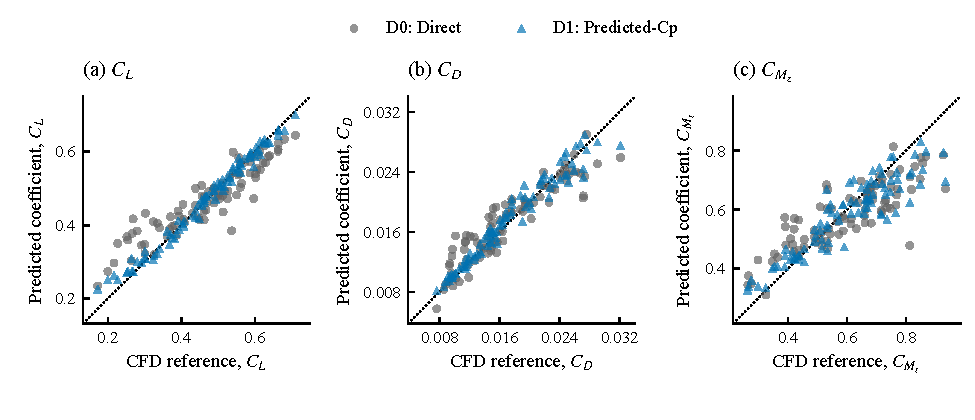
\includegraphics[width=0.96\textwidth]{V_Results_and_Discussion/figures/V_E_Fig26/V_E_Fig26_ve_force_parity.pdf}
    \caption{Predicted versus CFD-reference (a) lift, (b) drag, and (c) pitching-moment coefficients for D0 and D1 at $N=20$. Each point represents one of 88 test wings, with predictions averaged over three training subsets.}
    \label{fig:ve-force-parity}
\end{figure*}



\subsection{Aerodynamic Coefficient Prediction Performance}
\label{subsec:aerodynamic-coefficient-prediction}

Accurate reconstruction of the surface pressure field does not, by itself, guarantee accurate prediction of integrated aerodynamic coefficients. The latter requires a downstream model to extract the load-relevant information from a high-dimensional pressure representation. The force-label efficiency of this representation is examined using three coefficient-regression strategies: direct regression from geometry and flow conditions (D0), regression conditioned on the pressure field predicted by the fixed M2 model (D1), and regression conditioned on CFD-reference pressure (D2). Separate regressors are trained for the lift coefficient $C_L$, drag coefficient $C_D$, and pitching-moment coefficient $C_{M_z}$. Seven force-label budgets, $N=10$, 20, 30, 40, 50, 80, and 100 wings, are considered, with three independently sampled training subsets at each budget. All reported errors are evaluated on the same 88 test wings. Here $N$ denotes the number of wings used to train the downstream coefficient regressors; the pressure supervision previously used to establish the fixed M2 model is not included in this budget. Figure~\ref{fig:ve-force-mae} shows the mean absolute error (MAE) across the seven budgets, and Table~\ref{tab:ve-force-mae} provides the corresponding numerical comparisons.

\begin{figure*}[!t]
    \centering
    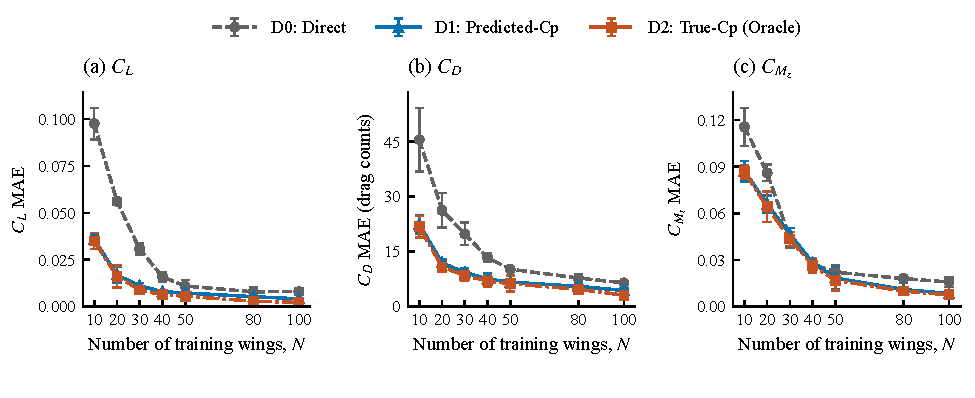
\includegraphics[width=0.96\textwidth]{V_Results_and_Discussion/figures/V_E_Fig25/V_E_Fig25_ve_force_mae.pdf}
    \caption{Force-coefficient MAE versus training size: (a) $C_L$, (b) $C_D$, and (c) $C_{M_z}$. D0, D1, and D2 use geometry/flow, M2-predicted pressure, and CFD pressure, respectively .}
    \label{fig:ve-force-mae}
\end{figure*}

The pressure-conditioned model provides its largest practical benefit at low force-label budgets. At $N=20$, the MAEs of D0 for $C_L$, $C_D$, and $C_{M_z}$ are 0.05610, 26.27 drag counts, and 0.08609, respectively. With M2-predicted pressure as additional input, D1 reduces these values to 0.01680, 11.88 drag counts, and 0.06592, corresponding to reductions of 70.1\%, 54.8\%, and 23.4\%. The improvement is strongest for lift, whose integrated response is directly related to the surface pressure loading. The reduction in drag-coefficient error is also substantial. By comparison, the smaller gain in pitching moment suggests a less favorable mapping from the available pressure representation to that particular integrated response; the present experiments do not isolate the physical origin of this difference.

Across the investigated budgets, the MAE generally decreases as more force-labeled wings become available, while the benefit of pressure conditioning remains coefficient-dependent. D1 outperforms D0 in mean MAE at all seven budgets for $C_L$ and $C_D$. For $C_{M_z}$, however, D1 is slightly less accurate at $N=30$ and 40: its MAEs are 0.04664 and 0.02833, compared with 0.04419 and 0.02746 for D0. At $N=100$, D1 reaches MAEs of 0.00414 for $C_L$, 4.39 drag counts for $C_D$, and 0.00838 for $C_{M_z}$. These results demonstrate that the contribution of the intermediate pressure field is not uniform across the three coefficients or training budgets.

The D2 results help distinguish the information supplied by pressure from the ability of the downstream regressor to use it. At $N=20$, replacing predicted pressure with CFD-reference pressure yields only modest additional reductions, to MAEs of 0.01611, 10.83 drag counts, and 0.06422 for $C_L$, $C_D$, and $C_{M_z}$, respectively. The separation becomes more apparent at $N=100$, where D2 achieves 0.00220, 3.12 drag counts, and 0.00755, compared with 0.00414, 4.39 drag counts, and 0.00838 for D1. Thus, additional pressure fidelity is more effectively reflected in the coefficient estimates when more force-labeled examples are available. This observation is consistent with a limitation imposed by downstream regression under very small training budgets, although the present comparison does not establish that explanation uniquely. Furthermore, D1 and D2 are fitted separately, so their difference cannot be attributed solely to M2 pressure error. Because D2 requires CFD-reference pressure as an input, it is a diagnostic reference rather than a deployable geometry-to-force surrogate.

The MAE over all 88 wings is complemented in Table~\ref{tab:ve-force-mae} by Best90 and Best80 MAE, which average the 80 and 71 lowest absolute errors, respectively, within each evaluated model. At $N=20$, D1 gives a drag MAE of 11.88 counts over all test wings, compared with Best90 and Best80 values of 8.98 and 7.30 counts. The corresponding D0 values are 26.27, 20.74, and 17.26 counts. Hence, the improvement from pressure conditioning is also evident over the lower-error majority of the test wings, rather than being restricted to changes in a few high-error cases. The gap between the full and trimmed means nevertheless indicates an uneven distribution of errors across wing configurations. Since the wings retained by the Best90 and Best80 definitions can differ between models, these statistics characterize error concentration and do not replace the full-set MAE.

\begin{table*}[!t]
    \centering
    \caption{Force-coefficient MAEs on 88 test wings, averaged over three training subsets.}
    \label{tab:ve-force-mae}
    \begingroup
    \fontsize{8.2}{9.8}\selectfont
    \setlength{\tabcolsep}{3.0pt}
    \renewcommand{\arraystretch}{1.06}

    \begin{tabular}{@{}r*{9}{c}@{}}
    \hline
    & \multicolumn{3}{c}{MAE}
    & \multicolumn{3}{c}{Best90 MAE}
    & \multicolumn{3}{c}{Best80 MAE} \\
    $N$ & D0 & D1 & D2
        & D0 & D1 & D2
        & D0 & D1 & D2 \\
    \hline

    \multicolumn{10}{@{}l}{\textit{$C_L$ (dimensionless)}} \\
    10  & 0.09764 & 0.03584 & 0.03501 & 0.08258 & 0.02785 & 0.02726 & 0.07027 & 0.02315 & 0.02260 \\
    20  & 0.05610 & 0.01680 & 0.01611 & 0.04473 & 0.01295 & 0.01211 & 0.03673 & 0.01055 & 0.00978 \\
    30  & 0.03067 & 0.01113 & 0.00889 & 0.02520 & 0.00903 & 0.00708 & 0.02082 & 0.00729 & 0.00568 \\
    40  & 0.01592 & 0.00791 & 0.00626 & 0.01263 & 0.00620 & 0.00484 & 0.01015 & 0.00511 & 0.00398 \\
    50  & 0.01095 & 0.00729 & 0.00557 & 0.00793 & 0.00563 & 0.00429 & 0.00647 & 0.00455 & 0.00346 \\
    80  & 0.00787 & 0.00529 & 0.00287 & 0.00558 & 0.00411 & 0.00218 & 0.00444 & 0.00347 & 0.00182 \\
    100 & 0.00800 & 0.00414 & 0.00220 & 0.00580 & 0.00335 & 0.00174 & 0.00478 & 0.00274 & 0.00145 \\

    \hline
    \multicolumn{10}{@{}l}{\textit{$C_D$ (drag counts)}} \\
    10  & 45.56 & 22.44 & 21.82 & 38.36 & 17.33 & 16.83 & 32.99 & 14.55 & 14.20 \\
    20  & 26.27 & 11.88 & 10.83 & 20.74 & 8.98 & 8.17 & 17.26 & 7.30 & 6.76 \\
    30  & 19.83 & 9.33 & 8.47 & 15.21 & 6.21 & 5.56 & 12.41 & 4.65 & 4.37 \\
    40  & 13.34 & 7.54 & 7.00 & 9.95 & 4.70 & 4.40 & 8.01 & 3.51 & 3.42 \\
    50  & 10.20 & 6.67 & 6.26 & 7.15 & 3.81 & 3.47 & 5.62 & 2.76 & 2.62 \\
    80  & 7.79 & 5.51 & 4.69 & 4.96 & 3.29 & 2.61 & 3.87 & 2.38 & 1.97 \\
    100 & 6.47 & 4.39 & 3.12 & 4.73 & 2.93 & 2.18 & 3.79 & 2.21 & 1.70 \\

    \hline
    \multicolumn{10}{@{}l}{\textit{$C_{M_z}$ (dimensionless)}} \\
    10  & 0.11566 & 0.08714 & 0.08674 & 0.09678 & 0.07124 & 0.07112 & 0.08294 & 0.05965 & 0.05956 \\
    20  & 0.08609 & 0.06592 & 0.06422 & 0.07016 & 0.05444 & 0.05251 & 0.06067 & 0.04643 & 0.04434 \\
    30  & 0.04419 & 0.04664 & 0.04351 & 0.03604 & 0.03874 & 0.03608 & 0.02976 & 0.03283 & 0.03051 \\
    40  & 0.02746 & 0.02833 & 0.02650 & 0.02139 & 0.02264 & 0.02140 & 0.01756 & 0.01881 & 0.01796 \\
    50  & 0.02210 & 0.01837 & 0.01695 & 0.01680 & 0.01481 & 0.01363 & 0.01394 & 0.01202 & 0.01136 \\
    80  & 0.01800 & 0.01098 & 0.00997 & 0.01326 & 0.00874 & 0.00826 & 0.01109 & 0.00735 & 0.00701 \\
    100 & 0.01574 & 0.00838 & 0.00755 & 0.01146 & 0.00681 & 0.00632 & 0.00984 & 0.00576 & 0.00537 \\

    \hline
    \end{tabular}
    \endgroup
\end{table*}

The representative small-sample case in Fig.~\ref{fig:ve-force-parity} provides a complementary view of the error distribution. At $N=20$, D1 predictions for lift and drag lie appreciably closer to the ideal agreement line than those of D0; the pitching-moment predictions remain more dispersed, consistent with their smaller relative MAE reduction. To prevent repeated evaluations of the same wing from appearing as independent observations, each plotted prediction is the arithmetic mean of the outputs from the three training-subset models for that wing. This averaging is used only for visualization: the metrics in Fig.~\ref{fig:ve-force-mae} and Table~\ref{tab:ve-force-mae} are calculated separately for each training subset before aggregation. Taken together, the results indicate that the fixed hierarchical pressure representation improves coefficient estimation when force labels are scarce, particularly for lift and drag, while leaving a coefficient-dependent residual error that is more apparent for challenging configurations.

\begin{figure*}[!t]
    \centering
    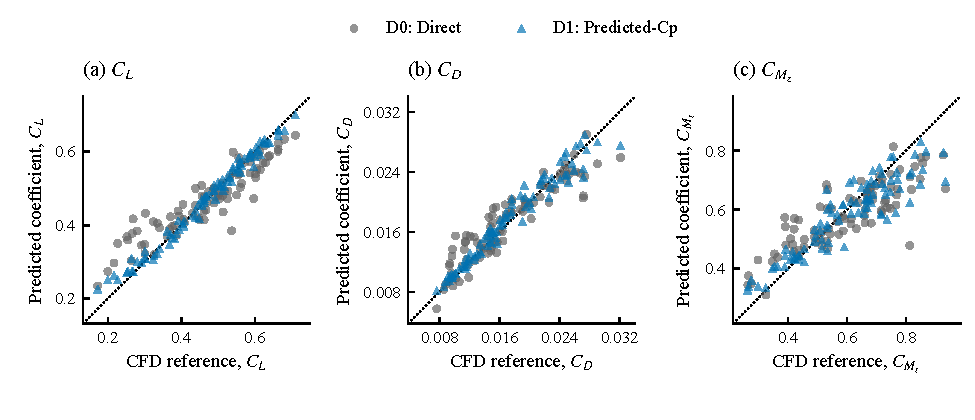
\includegraphics[width=0.96\textwidth]{V_Results_and_Discussion/figures/V_E_Fig26/V_E_Fig26_ve_force_parity.pdf}
    \caption{Predicted versus CFD-reference (a) lift, (b) drag, and (c) pitching-moment coefficients for D0 and D1 at $N=20$. Each point represents one of 88 test wings, with predictions averaged over three training subsets.}
    \label{fig:ve-force-parity}
\end{figure*}



\subsection{Aerodynamic Coefficient Prediction Performance}
\label{subsec:aerodynamic-coefficient-prediction}

Accurate reconstruction of the surface pressure field does not, by itself, guarantee accurate prediction of integrated aerodynamic coefficients. The latter requires a downstream model to extract the load-relevant information from a high-dimensional pressure representation. The force-label efficiency of this representation is examined using three coefficient-regression strategies: direct regression from geometry and flow conditions (D0), regression conditioned on the pressure field predicted by the fixed M2 model (D1), and regression conditioned on CFD-reference pressure (D2). Separate regressors are trained for the lift coefficient $C_L$, drag coefficient $C_D$, and pitching-moment coefficient $C_{M_z}$. Seven force-label budgets, $N=10$, 20, 30, 40, 50, 80, and 100 wings, are considered, with three independently sampled training subsets at each budget. All reported errors are evaluated on the same 88 test wings. Here $N$ denotes the number of wings used to train the downstream coefficient regressors; the pressure supervision previously used to establish the fixed M2 model is not included in this budget. Figure~\ref{fig:ve-force-mae} shows the mean absolute error (MAE) across the seven budgets, and Table~\ref{tab:ve-force-mae} provides the corresponding numerical comparisons.

\begin{figure*}[!t]
    \centering
    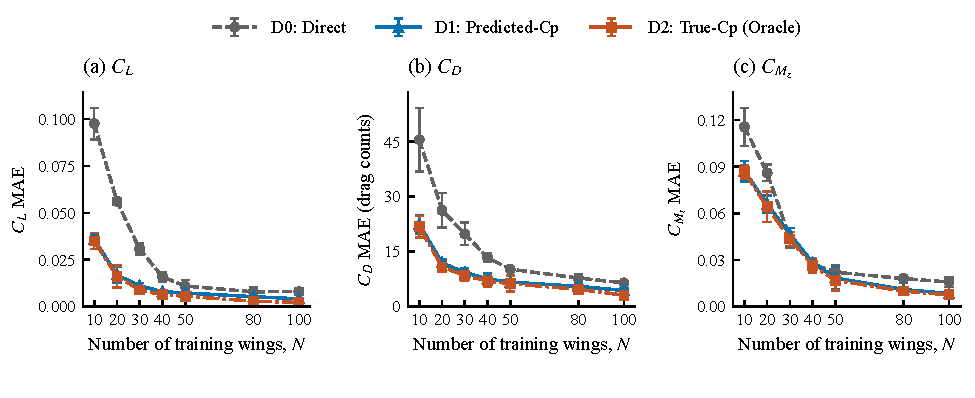
\includegraphics[width=0.96\textwidth]{V_Results_and_Discussion/figures/V_E_Fig25/V_E_Fig25_ve_force_mae.pdf}
    \caption{Force-coefficient MAE versus training size: (a) $C_L$, (b) $C_D$, and (c) $C_{M_z}$. D0, D1, and D2 use geometry/flow, M2-predicted pressure, and CFD pressure, respectively .}
    \label{fig:ve-force-mae}
\end{figure*}

The pressure-conditioned model provides its largest practical benefit at low force-label budgets. At $N=20$, the MAEs of D0 for $C_L$, $C_D$, and $C_{M_z}$ are 0.05610, 26.27 drag counts, and 0.08609, respectively. With M2-predicted pressure as additional input, D1 reduces these values to 0.01680, 11.88 drag counts, and 0.06592, corresponding to reductions of 70.1\%, 54.8\%, and 23.4\%. The improvement is strongest for lift, whose integrated response is directly related to the surface pressure loading. The reduction in drag-coefficient error is also substantial. By comparison, the smaller gain in pitching moment suggests a less favorable mapping from the available pressure representation to that particular integrated response; the present experiments do not isolate the physical origin of this difference.

Across the investigated budgets, the MAE generally decreases as more force-labeled wings become available, while the benefit of pressure conditioning remains coefficient-dependent. D1 outperforms D0 in mean MAE at all seven budgets for $C_L$ and $C_D$. For $C_{M_z}$, however, D1 is slightly less accurate at $N=30$ and 40: its MAEs are 0.04664 and 0.02833, compared with 0.04419 and 0.02746 for D0. At $N=100$, D1 reaches MAEs of 0.00414 for $C_L$, 4.39 drag counts for $C_D$, and 0.00838 for $C_{M_z}$. These results demonstrate that the contribution of the intermediate pressure field is not uniform across the three coefficients or training budgets.

The D2 results help distinguish the information supplied by pressure from the ability of the downstream regressor to use it. At $N=20$, replacing predicted pressure with CFD-reference pressure yields only modest additional reductions, to MAEs of 0.01611, 10.83 drag counts, and 0.06422 for $C_L$, $C_D$, and $C_{M_z}$, respectively. The separation becomes more apparent at $N=100$, where D2 achieves 0.00220, 3.12 drag counts, and 0.00755, compared with 0.00414, 4.39 drag counts, and 0.00838 for D1. Thus, additional pressure fidelity is more effectively reflected in the coefficient estimates when more force-labeled examples are available. This observation is consistent with a limitation imposed by downstream regression under very small training budgets, although the present comparison does not establish that explanation uniquely. Furthermore, D1 and D2 are fitted separately, so their difference cannot be attributed solely to M2 pressure error. Because D2 requires CFD-reference pressure as an input, it is a diagnostic reference rather than a deployable geometry-to-force surrogate.

The MAE over all 88 wings is complemented in Table~\ref{tab:ve-force-mae} by Best90 and Best80 MAE, which average the 80 and 71 lowest absolute errors, respectively, within each evaluated model. At $N=20$, D1 gives a drag MAE of 11.88 counts over all test wings, compared with Best90 and Best80 values of 8.98 and 7.30 counts. The corresponding D0 values are 26.27, 20.74, and 17.26 counts. Hence, the improvement from pressure conditioning is also evident over the lower-error majority of the test wings, rather than being restricted to changes in a few high-error cases. The gap between the full and trimmed means nevertheless indicates an uneven distribution of errors across wing configurations. Since the wings retained by the Best90 and Best80 definitions can differ between models, these statistics characterize error concentration and do not replace the full-set MAE.

\begin{table*}[!t]
    \centering
    \caption{Force-coefficient MAEs on 88 test wings, averaged over three training subsets.}
    \label{tab:ve-force-mae}
    \begingroup
    \fontsize{8.2}{9.8}\selectfont
    \setlength{\tabcolsep}{3.0pt}
    \renewcommand{\arraystretch}{1.06}

    \begin{tabular}{@{}r*{9}{c}@{}}
    \hline
    & \multicolumn{3}{c}{MAE}
    & \multicolumn{3}{c}{Best90 MAE}
    & \multicolumn{3}{c}{Best80 MAE} \\
    $N$ & D0 & D1 & D2
        & D0 & D1 & D2
        & D0 & D1 & D2 \\
    \hline

    \multicolumn{10}{@{}l}{\textit{$C_L$ (dimensionless)}} \\
    10  & 0.09764 & 0.03584 & 0.03501 & 0.08258 & 0.02785 & 0.02726 & 0.07027 & 0.02315 & 0.02260 \\
    20  & 0.05610 & 0.01680 & 0.01611 & 0.04473 & 0.01295 & 0.01211 & 0.03673 & 0.01055 & 0.00978 \\
    30  & 0.03067 & 0.01113 & 0.00889 & 0.02520 & 0.00903 & 0.00708 & 0.02082 & 0.00729 & 0.00568 \\
    40  & 0.01592 & 0.00791 & 0.00626 & 0.01263 & 0.00620 & 0.00484 & 0.01015 & 0.00511 & 0.00398 \\
    50  & 0.01095 & 0.00729 & 0.00557 & 0.00793 & 0.00563 & 0.00429 & 0.00647 & 0.00455 & 0.00346 \\
    80  & 0.00787 & 0.00529 & 0.00287 & 0.00558 & 0.00411 & 0.00218 & 0.00444 & 0.00347 & 0.00182 \\
    100 & 0.00800 & 0.00414 & 0.00220 & 0.00580 & 0.00335 & 0.00174 & 0.00478 & 0.00274 & 0.00145 \\

    \hline
    \multicolumn{10}{@{}l}{\textit{$C_D$ (drag counts)}} \\
    10  & 45.56 & 22.44 & 21.82 & 38.36 & 17.33 & 16.83 & 32.99 & 14.55 & 14.20 \\
    20  & 26.27 & 11.88 & 10.83 & 20.74 & 8.98 & 8.17 & 17.26 & 7.30 & 6.76 \\
    30  & 19.83 & 9.33 & 8.47 & 15.21 & 6.21 & 5.56 & 12.41 & 4.65 & 4.37 \\
    40  & 13.34 & 7.54 & 7.00 & 9.95 & 4.70 & 4.40 & 8.01 & 3.51 & 3.42 \\
    50  & 10.20 & 6.67 & 6.26 & 7.15 & 3.81 & 3.47 & 5.62 & 2.76 & 2.62 \\
    80  & 7.79 & 5.51 & 4.69 & 4.96 & 3.29 & 2.61 & 3.87 & 2.38 & 1.97 \\
    100 & 6.47 & 4.39 & 3.12 & 4.73 & 2.93 & 2.18 & 3.79 & 2.21 & 1.70 \\

    \hline
    \multicolumn{10}{@{}l}{\textit{$C_{M_z}$ (dimensionless)}} \\
    10  & 0.11566 & 0.08714 & 0.08674 & 0.09678 & 0.07124 & 0.07112 & 0.08294 & 0.05965 & 0.05956 \\
    20  & 0.08609 & 0.06592 & 0.06422 & 0.07016 & 0.05444 & 0.05251 & 0.06067 & 0.04643 & 0.04434 \\
    30  & 0.04419 & 0.04664 & 0.04351 & 0.03604 & 0.03874 & 0.03608 & 0.02976 & 0.03283 & 0.03051 \\
    40  & 0.02746 & 0.02833 & 0.02650 & 0.02139 & 0.02264 & 0.02140 & 0.01756 & 0.01881 & 0.01796 \\
    50  & 0.02210 & 0.01837 & 0.01695 & 0.01680 & 0.01481 & 0.01363 & 0.01394 & 0.01202 & 0.01136 \\
    80  & 0.01800 & 0.01098 & 0.00997 & 0.01326 & 0.00874 & 0.00826 & 0.01109 & 0.00735 & 0.00701 \\
    100 & 0.01574 & 0.00838 & 0.00755 & 0.01146 & 0.00681 & 0.00632 & 0.00984 & 0.00576 & 0.00537 \\

    \hline
    \end{tabular}
    \endgroup
\end{table*}

The representative small-sample case in Fig.~\ref{fig:ve-force-parity} provides a complementary view of the error distribution. At $N=20$, D1 predictions for lift and drag lie appreciably closer to the ideal agreement line than those of D0; the pitching-moment predictions remain more dispersed, consistent with their smaller relative MAE reduction. To prevent repeated evaluations of the same wing from appearing as independent observations, each plotted prediction is the arithmetic mean of the outputs from the three training-subset models for that wing. This averaging is used only for visualization: the metrics in Fig.~\ref{fig:ve-force-mae} and Table~\ref{tab:ve-force-mae} are calculated separately for each training subset before aggregation. Taken together, the results indicate that the fixed hierarchical pressure representation improves coefficient estimation when force labels are scarce, particularly for lift and drag, while leaving a coefficient-dependent residual error that is more apparent for challenging configurations.

\begin{figure*}[!t]
    \centering
    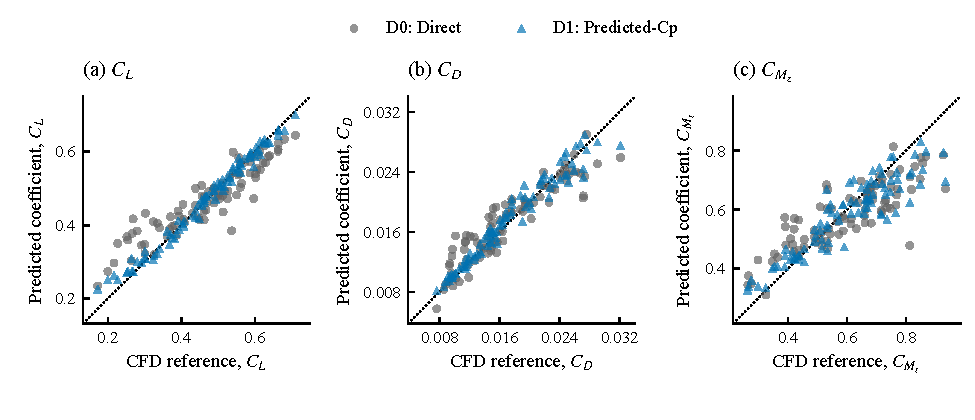
\includegraphics[width=0.96\textwidth]{V_Results_and_Discussion/figures/V_E_Fig26/V_E_Fig26_ve_force_parity.pdf}
    \caption{Predicted versus CFD-reference (a) lift, (b) drag, and (c) pitching-moment coefficients for D0 and D1 at $N=20$. Each point represents one of 88 test wings, with predictions averaged over three training subsets.}
    \label{fig:ve-force-parity}
\end{figure*}



\subsection{Aerodynamic Coefficient Prediction Performance}
\label{subsec:aerodynamic-coefficient-prediction}

Accurate reconstruction of the surface pressure field does not, by itself, guarantee accurate prediction of integrated aerodynamic coefficients. The latter requires a downstream model to extract the load-relevant information from a high-dimensional pressure representation. The force-label efficiency of this representation is examined using three coefficient-regression strategies: direct regression from geometry and flow conditions (D0), regression conditioned on the pressure field predicted by the fixed M2 model (D1), and regression conditioned on CFD-reference pressure (D2). Separate regressors are trained for the lift coefficient $C_L$, drag coefficient $C_D$, and pitching-moment coefficient $C_{M_z}$. Seven force-label budgets, $N=10$, 20, 30, 40, 50, 80, and 100 wings, are considered, with three independently sampled training subsets at each budget. All reported errors are evaluated on the same 88 test wings. Here $N$ denotes the number of wings used to train the downstream coefficient regressors; the pressure supervision previously used to establish the fixed M2 model is not included in this budget. Figure~\ref{fig:ve-force-mae} shows the mean absolute error (MAE) across the seven budgets, and Table~\ref{tab:ve-force-mae} provides the corresponding numerical comparisons.

\begin{figure*}[!t]
    \centering
    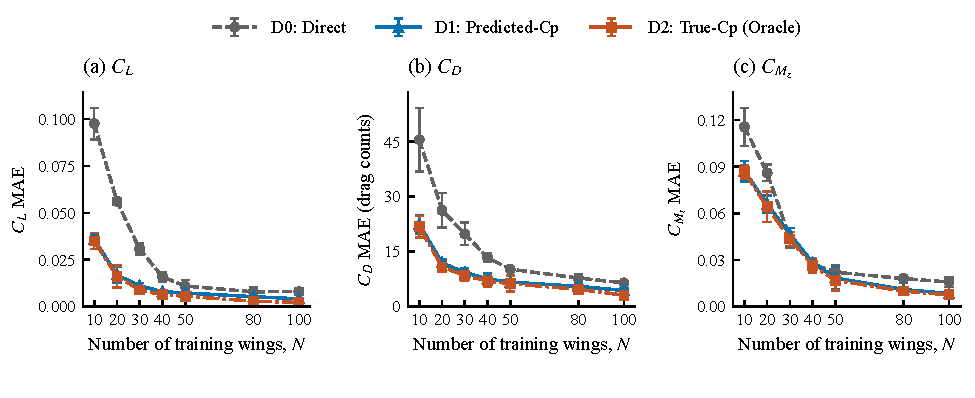
\includegraphics[width=0.96\textwidth]{V_Results_and_Discussion/figures/V_E_Fig25/V_E_Fig25_ve_force_mae.pdf}
    \caption{Force-coefficient MAE versus training size: (a) $C_L$, (b) $C_D$, and (c) $C_{M_z}$. D0, D1, and D2 use geometry/flow, M2-predicted pressure, and CFD pressure, respectively .}
    \label{fig:ve-force-mae}
\end{figure*}

The pressure-conditioned model provides its largest practical benefit at low force-label budgets. At $N=20$, the MAEs of D0 for $C_L$, $C_D$, and $C_{M_z}$ are 0.05610, 26.27 drag counts, and 0.08609, respectively. With M2-predicted pressure as additional input, D1 reduces these values to 0.01680, 11.88 drag counts, and 0.06592, corresponding to reductions of 70.1\%, 54.8\%, and 23.4\%. The improvement is strongest for lift, whose integrated response is directly related to the surface pressure loading. The reduction in drag-coefficient error is also substantial. By comparison, the smaller gain in pitching moment suggests a less favorable mapping from the available pressure representation to that particular integrated response; the present experiments do not isolate the physical origin of this difference.

Across the investigated budgets, the MAE generally decreases as more force-labeled wings become available, while the benefit of pressure conditioning remains coefficient-dependent. D1 outperforms D0 in mean MAE at all seven budgets for $C_L$ and $C_D$. For $C_{M_z}$, however, D1 is slightly less accurate at $N=30$ and 40: its MAEs are 0.04664 and 0.02833, compared with 0.04419 and 0.02746 for D0. At $N=100$, D1 reaches MAEs of 0.00414 for $C_L$, 4.39 drag counts for $C_D$, and 0.00838 for $C_{M_z}$. These results demonstrate that the contribution of the intermediate pressure field is not uniform across the three coefficients or training budgets.

The D2 results help distinguish the information supplied by pressure from the ability of the downstream regressor to use it. At $N=20$, replacing predicted pressure with CFD-reference pressure yields only modest additional reductions, to MAEs of 0.01611, 10.83 drag counts, and 0.06422 for $C_L$, $C_D$, and $C_{M_z}$, respectively. The separation becomes more apparent at $N=100$, where D2 achieves 0.00220, 3.12 drag counts, and 0.00755, compared with 0.00414, 4.39 drag counts, and 0.00838 for D1. Thus, additional pressure fidelity is more effectively reflected in the coefficient estimates when more force-labeled examples are available. This observation is consistent with a limitation imposed by downstream regression under very small training budgets, although the present comparison does not establish that explanation uniquely. Furthermore, D1 and D2 are fitted separately, so their difference cannot be attributed solely to M2 pressure error. Because D2 requires CFD-reference pressure as an input, it is a diagnostic reference rather than a deployable geometry-to-force surrogate.

The MAE over all 88 wings is complemented in Table~\ref{tab:ve-force-mae} by Best90 and Best80 MAE, which average the 80 and 71 lowest absolute errors, respectively, within each evaluated model. At $N=20$, D1 gives a drag MAE of 11.88 counts over all test wings, compared with Best90 and Best80 values of 8.98 and 7.30 counts. The corresponding D0 values are 26.27, 20.74, and 17.26 counts. Hence, the improvement from pressure conditioning is also evident over the lower-error majority of the test wings, rather than being restricted to changes in a few high-error cases. The gap between the full and trimmed means nevertheless indicates an uneven distribution of errors across wing configurations. Since the wings retained by the Best90 and Best80 definitions can differ between models, these statistics characterize error concentration and do not replace the full-set MAE.

\begin{table*}[!t]
    \centering
    \caption{Force-coefficient MAEs on 88 test wings, averaged over three training subsets.}
    \label{tab:ve-force-mae}
    \begingroup
    \fontsize{8.2}{9.8}\selectfont
    \setlength{\tabcolsep}{3.0pt}
    \renewcommand{\arraystretch}{1.06}

    \begin{tabular}{@{}r*{9}{c}@{}}
    \hline
    & \multicolumn{3}{c}{MAE}
    & \multicolumn{3}{c}{Best90 MAE}
    & \multicolumn{3}{c}{Best80 MAE} \\
    $N$ & D0 & D1 & D2
        & D0 & D1 & D2
        & D0 & D1 & D2 \\
    \hline

    \multicolumn{10}{@{}l}{\textit{$C_L$ (dimensionless)}} \\
    10  & 0.09764 & 0.03584 & 0.03501 & 0.08258 & 0.02785 & 0.02726 & 0.07027 & 0.02315 & 0.02260 \\
    20  & 0.05610 & 0.01680 & 0.01611 & 0.04473 & 0.01295 & 0.01211 & 0.03673 & 0.01055 & 0.00978 \\
    30  & 0.03067 & 0.01113 & 0.00889 & 0.02520 & 0.00903 & 0.00708 & 0.02082 & 0.00729 & 0.00568 \\
    40  & 0.01592 & 0.00791 & 0.00626 & 0.01263 & 0.00620 & 0.00484 & 0.01015 & 0.00511 & 0.00398 \\
    50  & 0.01095 & 0.00729 & 0.00557 & 0.00793 & 0.00563 & 0.00429 & 0.00647 & 0.00455 & 0.00346 \\
    80  & 0.00787 & 0.00529 & 0.00287 & 0.00558 & 0.00411 & 0.00218 & 0.00444 & 0.00347 & 0.00182 \\
    100 & 0.00800 & 0.00414 & 0.00220 & 0.00580 & 0.00335 & 0.00174 & 0.00478 & 0.00274 & 0.00145 \\

    \hline
    \multicolumn{10}{@{}l}{\textit{$C_D$ (drag counts)}} \\
    10  & 45.56 & 22.44 & 21.82 & 38.36 & 17.33 & 16.83 & 32.99 & 14.55 & 14.20 \\
    20  & 26.27 & 11.88 & 10.83 & 20.74 & 8.98 & 8.17 & 17.26 & 7.30 & 6.76 \\
    30  & 19.83 & 9.33 & 8.47 & 15.21 & 6.21 & 5.56 & 12.41 & 4.65 & 4.37 \\
    40  & 13.34 & 7.54 & 7.00 & 9.95 & 4.70 & 4.40 & 8.01 & 3.51 & 3.42 \\
    50  & 10.20 & 6.67 & 6.26 & 7.15 & 3.81 & 3.47 & 5.62 & 2.76 & 2.62 \\
    80  & 7.79 & 5.51 & 4.69 & 4.96 & 3.29 & 2.61 & 3.87 & 2.38 & 1.97 \\
    100 & 6.47 & 4.39 & 3.12 & 4.73 & 2.93 & 2.18 & 3.79 & 2.21 & 1.70 \\

    \hline
    \multicolumn{10}{@{}l}{\textit{$C_{M_z}$ (dimensionless)}} \\
    10  & 0.11566 & 0.08714 & 0.08674 & 0.09678 & 0.07124 & 0.07112 & 0.08294 & 0.05965 & 0.05956 \\
    20  & 0.08609 & 0.06592 & 0.06422 & 0.07016 & 0.05444 & 0.05251 & 0.06067 & 0.04643 & 0.04434 \\
    30  & 0.04419 & 0.04664 & 0.04351 & 0.03604 & 0.03874 & 0.03608 & 0.02976 & 0.03283 & 0.03051 \\
    40  & 0.02746 & 0.02833 & 0.02650 & 0.02139 & 0.02264 & 0.02140 & 0.01756 & 0.01881 & 0.01796 \\
    50  & 0.02210 & 0.01837 & 0.01695 & 0.01680 & 0.01481 & 0.01363 & 0.01394 & 0.01202 & 0.01136 \\
    80  & 0.01800 & 0.01098 & 0.00997 & 0.01326 & 0.00874 & 0.00826 & 0.01109 & 0.00735 & 0.00701 \\
    100 & 0.01574 & 0.00838 & 0.00755 & 0.01146 & 0.00681 & 0.00632 & 0.00984 & 0.00576 & 0.00537 \\

    \hline
    \end{tabular}
    \endgroup
\end{table*}

The representative small-sample case in Fig.~\ref{fig:ve-force-parity} provides a complementary view of the error distribution. At $N=20$, D1 predictions for lift and drag lie appreciably closer to the ideal agreement line than those of D0; the pitching-moment predictions remain more dispersed, consistent with their smaller relative MAE reduction. To prevent repeated evaluations of the same wing from appearing as independent observations, each plotted prediction is the arithmetic mean of the outputs from the three training-subset models for that wing. This averaging is used only for visualization: the metrics in Fig.~\ref{fig:ve-force-mae} and Table~\ref{tab:ve-force-mae} are calculated separately for each training subset before aggregation. Taken together, the results indicate that the fixed hierarchical pressure representation improves coefficient estimation when force labels are scarce, particularly for lift and drag, while leaving a coefficient-dependent residual error that is more apparent for challenging configurations.

\begin{figure*}[!t]
    \centering
    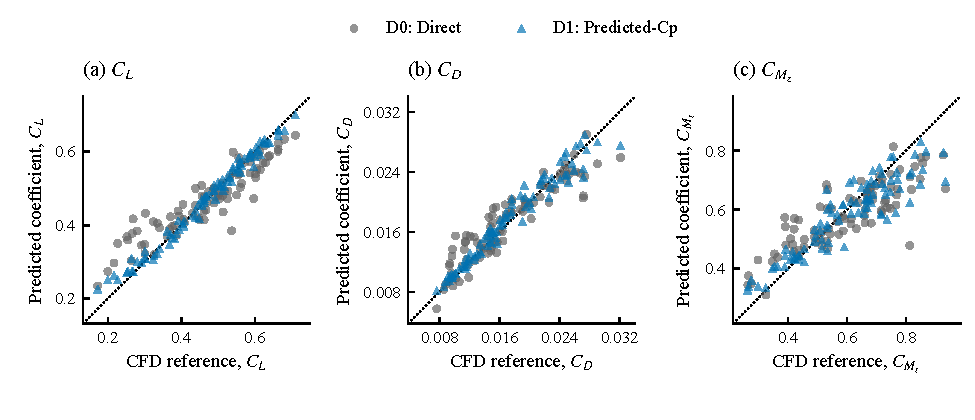
\includegraphics[width=0.96\textwidth]{V_Results_and_Discussion/figures/V_E_Fig26/V_E_Fig26_ve_force_parity.pdf}
    \caption{Predicted versus CFD-reference (a) lift, (b) drag, and (c) pitching-moment coefficients for D0 and D1 at $N=20$. Each point represents one of 88 test wings, with predictions averaged over three training subsets.}
    \label{fig:ve-force-parity}
\end{figure*}

